\documentclass[11pt,a4paper]{article}

\usepackage{Act}
\usepackage{listings}

\begin{document}
\input{\detokenize{/home/fenarius/Travail/Cours/Commun/latex/Macros.tex}}

\DevoirNSI{Processus}{\Term}\vspace{0.2cm}
\pythonmode
%Nom de la première activité
Cet exercice pourra utiliser des commandes de systèmes d'exploitation de type {\sc unix} telles que {\tt cd, ls, mkdir, rm, mv, cat}
\QListe
\item Dans un système d'exploitation de type {\sc unix}, on considère l'arborescence des fichiers suivante dans laquelle les noms de dossiers sont en italique et ceux des fichiers sont en gras : \\
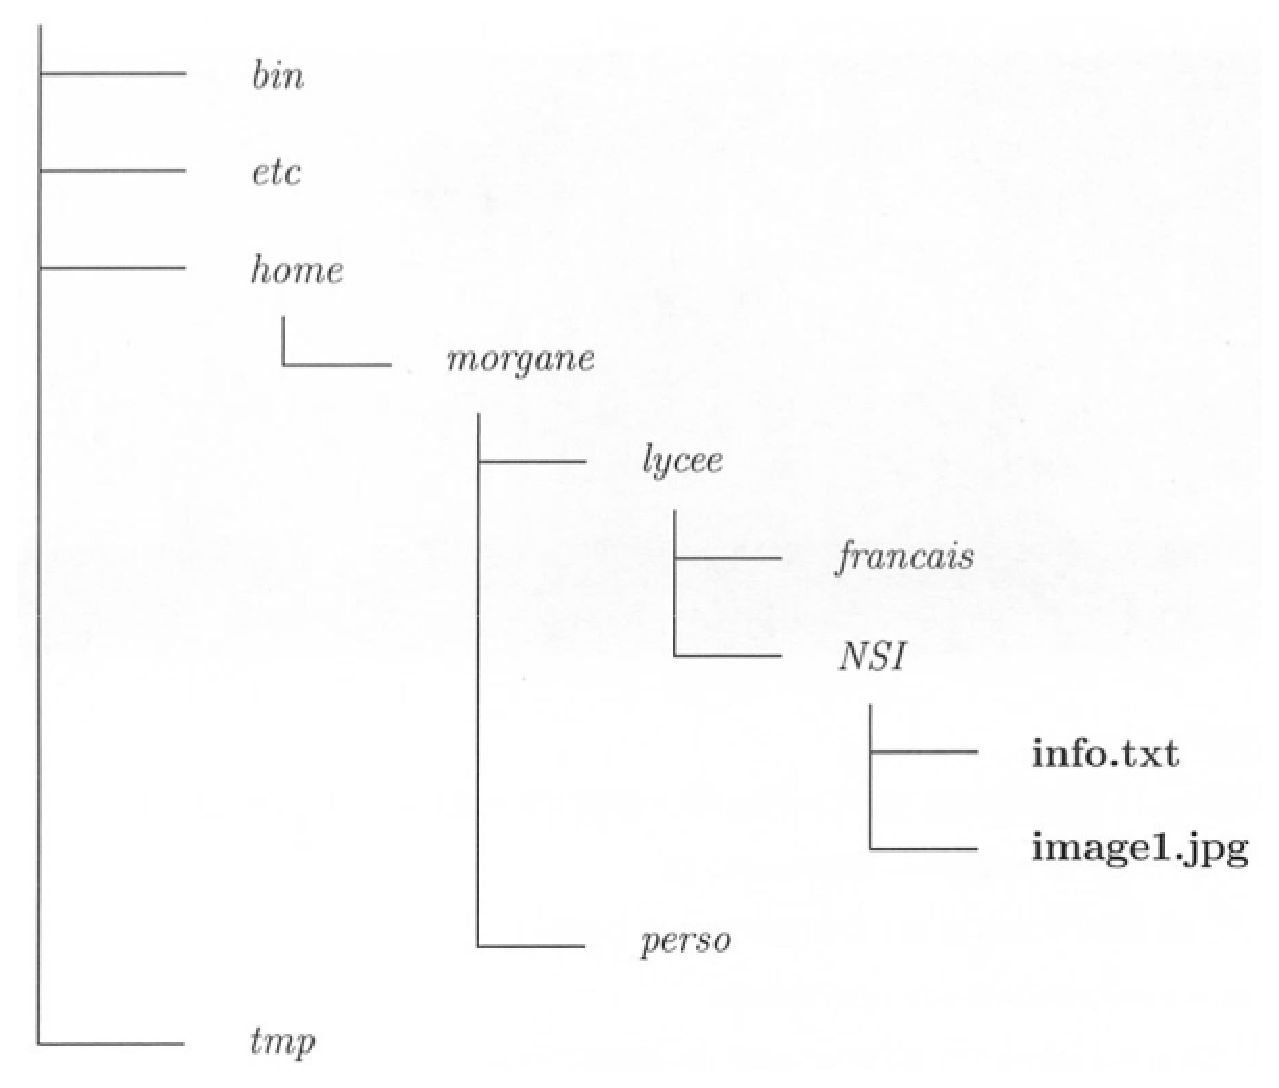
\includegraphics[width=250px]{C4-arbo.eps}

On suppose qu'on se trouve actuellement dans le dossier {\tt /home/morgane}
\SQListe
\item Quel sera l'affichage produit par la commande {\tt ls} ?
\item Ecrire la commande qui permet, à partir de cet emplacement, d'atteindre le répertoire {\tt lycee}
\item Ecrire la commande qui permet de créer à cet emplacement un répertoire nommé {\tt algorithmique}
\item Ecrire la commande qui permet, à partir de cet emplacement de supprimer le fichier {\tt image1.jpg}
\FinListe
\item Sur les processus
\SQListe
\item Donner la definition d'un processus.
\item Donner le nom de la commande permettant de lister les processus en cours d'exécution.
\item  Voici un extrait de l'affichage des processus fonctionnant sur un ordinateur : \\
\begin{tabular}{>{\tt}l>{\tt}l>{\tt}l>{\tt}l>{\tt}l>{\tt}l>{\tt}l>{\tt}l}
UID & PID & PPID & C & STIME & TTY & TIME & CMD \\ 
fenarius &   3118 &   2226 & 0 &09:49 &?    &    00:00:00 & /usr/libexec/gvfsd-metadata \\
fenarius &   3318 &   2454 & 0 &09:49 &?    &    00:00:11 & /usr/lib/thunderbird/thunder \\
fenarius &   3617 &   2454 & 8 &09:49 &?    &    00:02:25 & /snap/firefox/2088/usr/lib/f \\
fenarius &   3721 &   2454 & 2 &09:49 &?    &    00:00:46 & /usr/bin/Xwayland :0 -rootle \\
fenarius &   3741 &   2226 & 0 &09:49 &?    &    00:00:00 & /usr/libexec/gsd-xsettings \\
fenarius &   3784 &   3318 & 0 &09:49 &?    &    00:00:00 & /usr/lib/thunderbird/thunder \\
fenarius &   3799 &   2226 & 0 &09:49 &?    &    00:00:00 & /usr/libexec/ibus-x11 \\
fenarius &   3853 &   2226 & 0 &09:49 &?    &    00:00:00 & /usr/libexec/gnome-terminal- \\
fenarius &   3887 &   3853 & 0 &09:49 &pts/0&    00:00:00 & bash \\
\end{tabular}
\item Que signifie {\tt PID} et {\tt PPID} ?
\item Citer deux processus ayant le même parent
\item Le client de messagerie {\tt thunderbird} est bloqué, quelle commande faut-il taper pour tuer ce processus ?
\FinListe
\item Ordonnancement des processus
Le tableau ci-dessous donne les demandes d'exécution de 4 processus. Plus la priorité est grande et plus le numéro de priorité est petit. Par exemple $P1$ (numéro de priorité 4) est \textbf{moins} prioritaire que $P2$ (numéro de priorité 2). On suppose que l'algorithme d'ordonnancement exécute à chaque instant le processus le plus prioritaire.
\SQListe
\item Reproduire et compléter le diagramme suivant en indiquant dans chaque case le processus exécuté. \\
\psset{unit=0.8cm}
    \psgrid[subgriddiv=0,gridlabels=0](0,-1)(14,0)
    \psaxes[labels=x,ticks=x]{-}(0,-1)(14,0)
    \rput(0.5,-0.5){P1}
\vspace{1.5cm}
\item On suppose que les processus $P1$, $P2$ et $P3$ ont besoin de ressources en accès exclusif pour fonctionner. Expliquer ce que signifie une situation d'interblocage et en donner un exemple.
\FinListe
\FinListe





\end{document}

